\chapter{\ac{lora} \ac{phy} Testing}

It has been repeatedly shown that \ac{lora} transmissions can be received at distances exceeding 10km in  unobstructed environments (free-space) when antennas are highly elevated \cite{3YP:LORA_RANGE_REVIEW}. However, these ideal radio conditions are unrealistic for swarm robots operating close to the ground in high-propagation environments such as forests. Therefore the first experiment in this paper identifies \ac{lora}'s physical performance and scenario specific limitations. Due to expected sparsity, only far field scenarios are relevant ($d_{\text{SP}\leftrightarrow \text{MP}} >  0.35$m).


\section{Methodology}
The purpose of this testing was to inform protocol decisions and assess capability of an off-the-shelf \ac{lora} \ac{phy}. A focus was taken to get enough data across a small selection of important scenarios and parameters to allow quantitively assessment. 

 The two main transmission environments selected were free-space and in-forest; this was to give an understanding of both low-propagation and high-propagation scenarios. Data collection was mainly spread over two locations: \textbf{$L_{A}$} and \textbf{$L_{B}$} (split into \textbf{$L_{B1}$} and \textbf{$L_{B2}$}), identified in Figure \ref{fig:new_forest_map} and \ref{fig:stansted_map} respectively. All locations were rural and therefore theoretically free from strong sources of external interference. Radio placement was decided by first placing the transmitting radio (slave) at a fixed location (\ac{sp}), and then, using the furthest receivable point as the starting point for the receiving radio (master). From there the master was positioned closer towards the slave for each future test (\ac{mp}). In each scenario the main interest was ground level transmissions; however, to assess whether radio performance was actually compromised by the placement, comparative measurements were taken with an elevated antenna. 
 
  \begin{figure}[H]
    \centering
    \includegraphics[width=\textwidth]{Figures/new_forest_light}
    \caption[Test Location: The New Forest, Hampshire, UK]{
    Test positions for \textbf{$L_A$} :  The New Forest, Hampshire, UK.\protect\footnotemark[1] \\
    \ac{sp} in open with \ac{los} to other points a combination of free-space and light vegetation. Exact positions are in Appendix \ref{sec:new_forest_test_pos}. To the left of \ac{mp}7 vegetation density increases,  making \ac{mp}7 the furthest position viable for free-space testing.
    }
    \label{fig:new_forest_map}
\end{figure}

\begingroup
 \begin{figure}[H]
    \centering
    \begin{tabular}{c}
    \subfloat[{
    Test positions for in-forest testing (\textbf{$L_{B1}$}). \ac{sp} in forest with \ac{los} to other points continually obstructed by a combination of leaved and bare trees. Exact positions are in Appendix \ref{sec:stansted_forest_test_pos}. Large clump of \ac{mp}s where radio reception was inconsistent.
    }]
    {\includegraphics[width=\textwidth]{Figures/stansted_forest}\label{fig:stansted_map_forest}} 
    \\
    \subfloat[{
        Test positions for free-space testing (\textbf{$L_{B2}$}). \ac{sp} in open with \ac{los} completely free-space. Exact positions are in Appendix \ref{sec:stansted_free_test_pos}. No access to right of \ac{mp}13.
    }]{\includegraphics[width=\textwidth]{Figures/stansted_free_space}\label{fig:stansted_map_free}}
    \end{tabular}
    \caption[Test Location: Stansted Forest, West Sussex, UK]{
    Test locations for \textbf{$L_B$} :  Stansted Forest, West Sussex, UK.\footnotemark[1]
    }
    \label{fig:stansted_map}
\end{figure}
\footnotetext[1]{
    	$\enskip $ Copyright © 2019 MapOSMatic/OCitySMap developers\\
    	\indent \indent $\enskip $ Map Data © 2019 OpenStreetMap contributors (see http://osm.org/copyright)\\
    	\indent \indent $\enskip $ British Style © MapQuest \\
    	\indent \indent $\enskip $ Contour Overlay © OpenSnowMap.org
}

 In terms of radio parameters, \ac{sf} was the main focus due to it being an on option mostly unique to \ac{lora}; all values were tested for this in all locations ($\text{\ac{sf}} = 7, 8, 9, 10$). Variations using the lowest (4/5) and highest (4/8) \ac{cr}s were collected to verify \ac{fec} performance. Additionally, as the maximum transmission unit is often defined by the protocol, the effects of varying packet length were taken (\ac{pl} = 20, 128, 255 [\ac{phy} limit]). The rest of the parameters were fixed. The 868.1MHz \ac{cf} was used with \ac{tp} set to 14dBm so that collected data would be relevant in regard to \ac{etsi} regulations. The bandwidth was fixed to 125kHz so that radio sensitivity was only affected by the \ac{sf}. The \ac{ps}s were set to 8 to match \ac{lorawan} \cite{3YP:LORAWAN_REGIONAL_PARAMS}. The number of packets (\ac{pc}) transmitted for each configuration was set to 50; though not guaranteed, this gave reasonable expectation of a normal distribution. See Table \ref{tab:TestDefinitions} for full test definitions.
 
 To test the point-to-point transmissions, two identical platforms, which together could log the performance of sending and receiving \ac{lora} transmissions, were required. The platforms had to be suitable for outdoor use, be able to test multiple radio configurations whilst on location and provide a mechanism to indicate to user when the maximum range had been reached. The hardware and corresponding software created for this purpose is detailed in Appendix \ref{sec:testing_platform}.
\begin{figure}[H]
    \centering
    \begin{tabular}{ccc}
    \subfloat[][$L_{A}$ : MP05 \\ (1.0m)]{\includegraphics[height=7.5cm]{Figures/la_MP5_H1_0}}
    \hspace{2.5mm}
    \subfloat[][$L_{B1}$ : SP \\ (0.5m)]{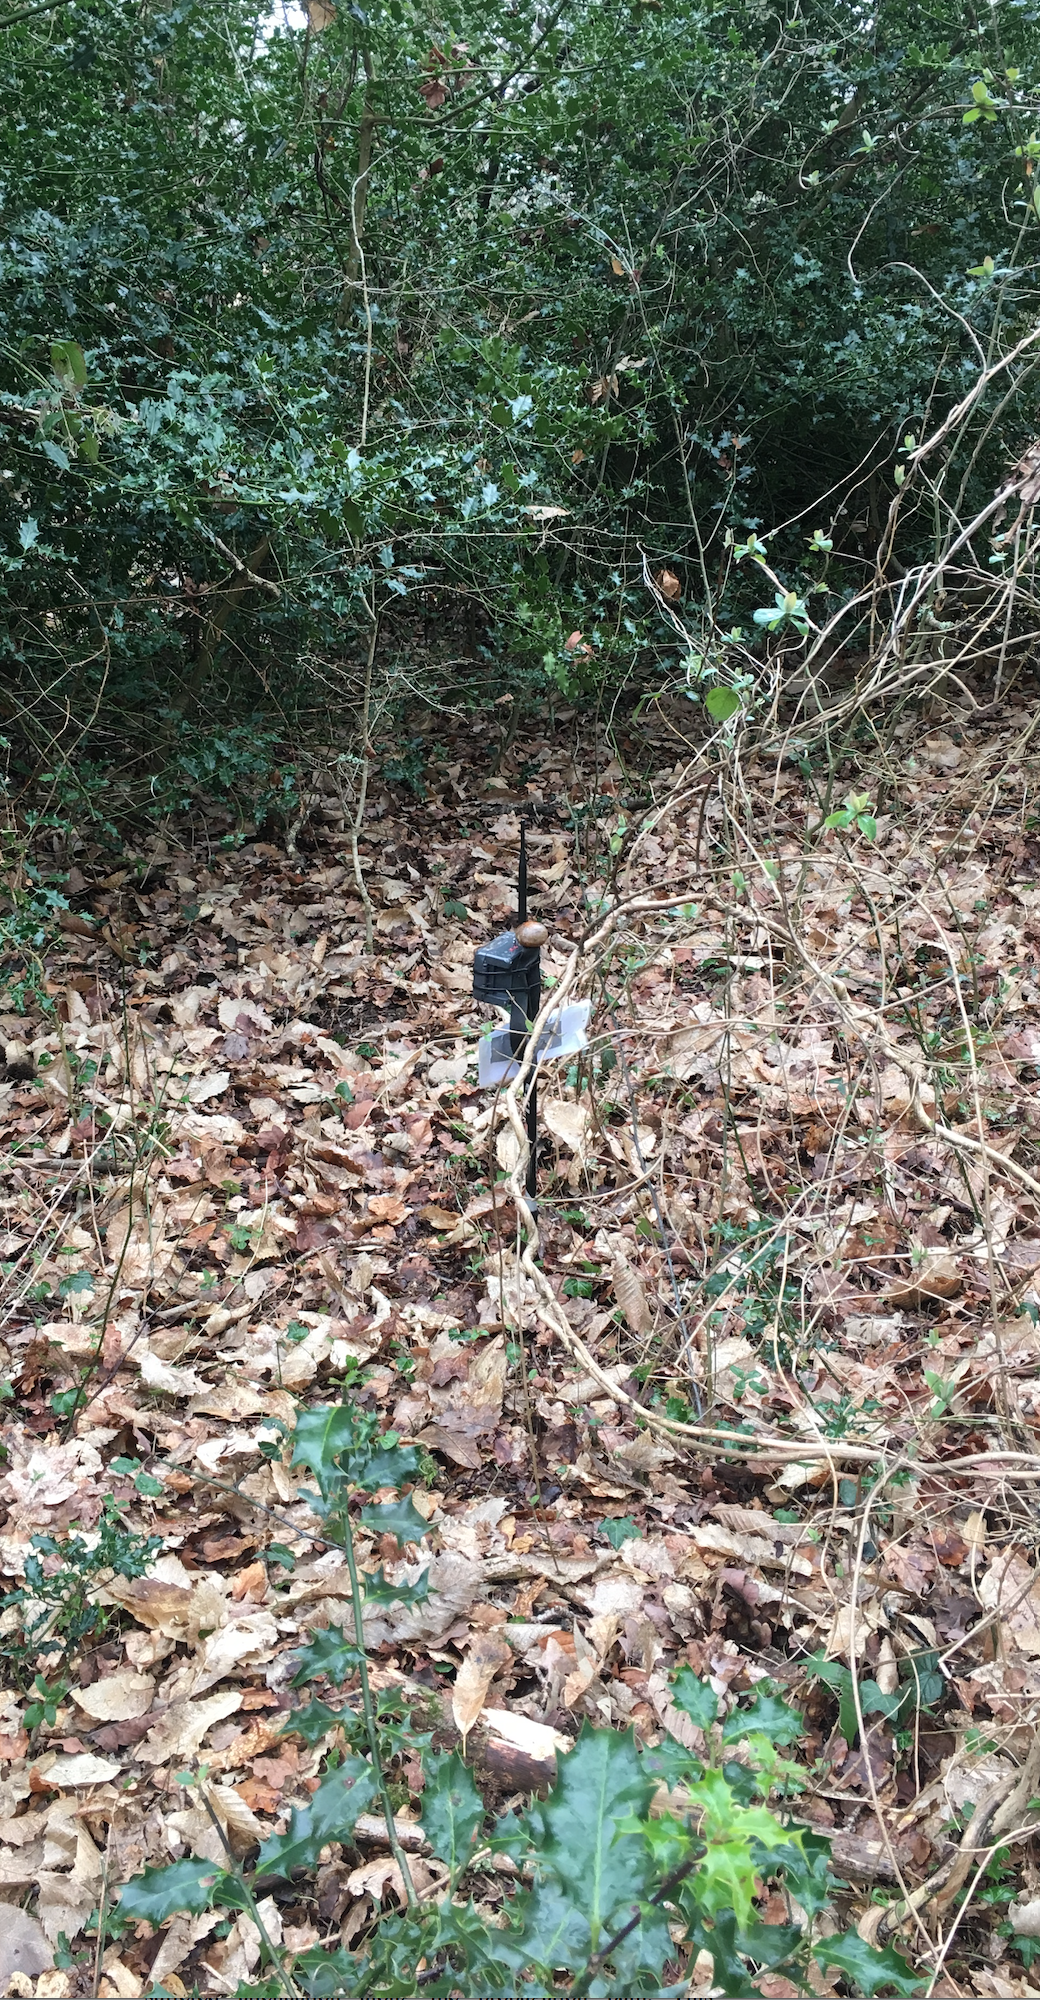
\includegraphics[height=7.5cm]{Figures/lb1_SP_H0_5}}
    \hspace{2.5mm}
    \subfloat[][$L_{B2}$ : MP16 \\ (0.0m)]{\includegraphics[height=7.5cm]{Figures/lb2_MP16_H0_0}}
    \end{tabular}
    \caption[Test location example]{Pictures of test environments and conditions. Although testing was split across multiple days at each location, the same dry conditions were present.}
    \label{fig:dataloggers}
\end{figure}
\endgroup
\vspace*{\fill}


 
\section{Test Platform}
\subsection{Hardware}
To test point-to-point transmissions, two identical platforms that could send and receive \ac{lora} transmissions were required. The basis of the designed test platform was HopeRF's\footnote{HopeRF Microelectronics Co. Ltd, China, https://www.hoperf.com/} RFM95W - a packet radio containing a \ac{lora} transceiver design licensed from Semtech; specifically, Adafruit's\footnote{Adafruit, USA, https://www.adafruit.com/} broken out version was used. As a raw packet radio, unlike the popular Microchip RN2483, it provided direct access to the radio interface. An omni-directional 3dBi 868MHz whip antenna was connected to the radio using a soldered uFL connector and a SMA to uFL connector. It was controlled by a Teensy\footnote{Teensy, https://www.pjrc.com/teensy/} 3.6 micro-controller, which also handled all logging responsibilities. A simple breakout circuit was designed and implemented on strip-board to connect the components in a condensed package. Each breakout board featured: a JST-PH2 battery connector, a coin cell holder for the Teensy's real-time-clock (\ac{rtc}), a power switch, a two-mode software switch, and three status LEDs. The schematic can be viewed in Figure \ref{fig:datalogger_schematic}. This was packaged to fit in an IP67 rated container with an internal 1800mAh \ac{lipo} battery. Switches and SMA antenna connectors were external; these were IP67 rated and extra sealing has been added where appropriate. The final dataloggers can be seen in Figure \ref{fig:dataloggers}. The Teensy is equipped with an SD card for storage but, due to cost considerations, a GPS module could not be implemented. The full breakdown of materials can be seen in Figure \ref{fig:datalogger_cost}.

\subsection{Software}
The system was designed such that one device (a slave) could be left unattended at a fixed location and controlled by a second device (a master); this was achieved using a command control system, as seen in Figure \ref{fig:software_cmd_system}. Two command classes were defined for testing purposes; these are as follows:
\begin{itemize}
	\item {\textbf{\texttt{HB\_CMD}}} : Command to trigger simple heartbeat functionality. When a slave receives this command it sends a heartbeat response (a short packet) on the base operating configuration. If in range, the master device will pick this up and alert the user.
	\item {\textbf{\texttt{TD\_CMD}}} : Command to trigger execution of a test definition (\ac{td}). In principle, the master device requests a set of packets to be sent by the slaves using the \ac{td} configuration; this is the basis of all test functionality. The full control flow is explained in detail in Figure \ref{fig:software_testdef_execution}.
\end{itemize}

%Whether a device was a master or a slave was determined by the board identifier stored in the Teensy EEPROM; this meant the same software could be flashed onto both, reducing the chance of software version inconsistencies.

\begin{figure}[H]
    \centering
    \includegraphics{Figures/software_cmd_system.pdf}
    \caption[Master-Slave command control method]{Diagram showing Master-Slave command control method.}
    \label{fig:software_cmd_system}
\end{figure}

\begin{figure}[H]
    \centering
    \includegraphics{Figures/software_testdef_execution.pdf}
    \caption[Master-Slave test definition execution method]{Diagram showing test definition execution.}
    \label{fig:software_testdef_execution}
\end{figure}




% the user, could trigger a command to be sent from the master to the receiver. 
%
%Whether a device was a master or a slave was determined by the board identifier stored in the Teensy EEPROM; this meant the same software could be flashed onto both, reducing the chance of software version inconsistencies.
%
% 
%Interfacing with the radio was handled by the RH\_RF95 driver from the Radiohead\footnote{Radiohead, https://www.airspayce.com/mikem/arduino/RadioHead/} library; this meant that only the control logic needed to be implemented. 
%
%
% A high-level overview of the planned test method is visualised in Figure \ref{master_slave_sequence}. \label{datalogger_software}
%
%
%    
%    Initial link testing will make use of two node classes: masters and slaves. The slaves are responsible for sending packets in the configuration requested by the master device. These are in the form of test definitions (TDs) that are stored on the master's memory card and will be processed one at a time. As the proposed system utilises only nodes, slave and master must have the same \ac{sf} and \ac{bw} for receiving the TD. This base state will be hard-coded such that the expected range exceeds or matches that of the longest range TD. The master will expect a certain number of packets (PC) from the slave, those received will have performance figures such as \ac{rssi}, \ac{snr} and \ac{per} recorded to the memory card under the specific test. The slave will wait for a new test definition once the PC has been sent. The master will proceed onto the next TD once the expected test length has expired.
\section{Results}
In total 498 test cases were executed, totalling 24,900 packet transmissions. Of this total 19,545 were successfully received (78.5\%). The distribution of receive conditions for these individual points is indicated by Figure \ref{fig:density_plot}. Note that the raw \ac{rssi} values returned by the Radiohead library, and therefore the datalogger, are in fact packet strength for the SX1276 module; therefore a post-processing step has been applied to get separate packet strength and \ac{rssi} values valid for the RFM95W module. For each test definition executed, the log-mean and log-standard deviations of the successfully received packet's: \ac{rssi}, \ac{snr}, and strength have been calculated.
\begin{figure}[H]
    \centering
   	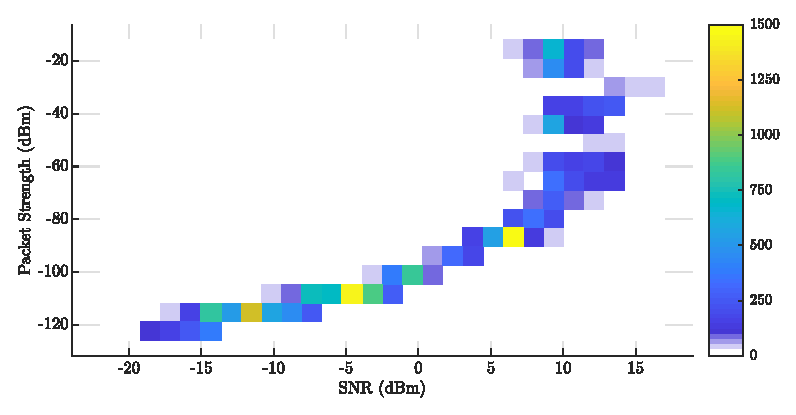
\includegraphics{Figures/density_plot}
    \caption[Test data distribution plot]{
    Density plot of received packet transmissions modelled as a bi-variate histogram with colour indicating received packet count. \\$Total\enskip Points = 19,545$
    }
    \label{fig:density_plot}
\end{figure}

\section{Discussion}
Some writing
\subsection{PHY Layer Performance}

\subsubsection{Spreading Factor}

\subsubsection{Coding Rate}

\subsubsection{Packet Length}

\begin{figure}[H]
    \centering
   	\includegraphics{Figures/snr_pp_separate_plot}
    \caption[Plots of \ac{snr} vs Packet Receive Percentage]{
   \ac{td} mean \ac{snr} values plotted against their packet receive percentages, separated by \ac{sf}s (Order = [[7, 8, 9], [10, 11, 12]]). For each \ac{sf} plot: the theoretical demodulation limit is indicated by the dotted line and the solid line corresponds to the best-fit sigmoid function; these are repeated in Figure \ref{fig:sf_pp_fit}. Although the best-fit sigmoids give a good representation of the general data pattern, and provide empirical demodulation cut-offs, they do not capture the high-variance receive behaviour when approaching the cut-off. This is reflected by the fact that only 62\%, 60\%, 66\%, 39\%, 77\% and 82\% of the respective training points fall inside the corresponding 95\% confidence interval. Notably \ac{sf}10 has very high-variance; this is reflected in the 95\% maximum receive chance. 
    }
    \label{fig:snr_pp_separate}
\end{figure}

\begin{figure}[H]
    \centering
   	\includegraphics{Figures/sf_fit_plot}
    \caption[Plot of sigmoid best-fits for \ac{snr} vs Packet Receive Percentage]{
    Plot of sigmoid best-fits generated in Figure \ref{fig:snr_pp_separate}. The plot clearly demonstrates the positive effect increasing \ac{sf} has on demodulation performance of the receiver. For \ac{sf}=7,8,9,10 demodulation success starts dropping approximately 2.5dBm before the theoretical limit ($D_L$), with a 50\% packet receive chance at $D_L$. This holds less so for \ac{sf}=11, for which drop-off starts around $D_L - 5dBm$, until $D_L$ where there is only a 10\% receive success. For \ac{sf}=12 drop-off starts around $D_L - 7.5dBm$, until $D_L$ where there is a 0\% receive success. Given that \ac{rssi} was relatively stable when $\ac{snr} < 0$, and that expected performance holds until a certain \ac{snr}, there is an indication that the sensitivity of the receiver is not as high as stated. 
     }
    \label{fig:sf_pp_fit}
\end{figure}

\subsection{Environmental Effects}
\subsubsection{Open (Free) Space}
High noise floor indicates that either the receiver's noise figure is not correct or there is more noise than expected in the environment. The fact that demodulation limit is nowhere near the true limit for SF10 onwards suggests that the cheaper radio does not perform correctly.
\subsubsection{Forest}
\subsubsection{Radio Height}
Increasing radio height massively increased range once reached 1m

% Distance in relatively open space (got)
% Distance in trees (got)
% Closeness to ground (got)
% Coding rate ??? (sort of got)
% Difference in slight movements (!!!)
%Lessons Learnt 
https://www.thethingsnetwork.org/forum/t/no-lower-rssi-than-121-dbm-possible-in-ttn/19890/15


\subsection{Open (Free) Space}
High noise floor indicates that either the receiver's noise figure is not correct or there is more noise than expected in the environment. The fact that demodulation limit is nowhere near the true limit for SF10 onwards suggests that the cheaper radio does not perform correctly.


\section{Discussion}

\subsection{Forest}
\subsection{Radio Height}

% Testing platform
% Testing methodology 
% Distance in relatively open space (got)
% Distance in trees (got)
% Closeness to ground (got)
% Coding rate ??? (sort of got)
% Difference in slight movements (!!!)
%Lessons Learnt 
https://www.thethingsnetwork.org/forum/t/no-lower-rssi-than-121-dbm-possible-in-ttn/19890/15